
\section{The Real Fourier Basis}

\par \indentt The amplitude-over-time function for a tone with fundamental frequency $\frac{1}{T}$ lives in $C[0,T]$, the space of continuous-time functions with period $T$. This information is not so helpful for musicians. Changing the function by adding terms or adjusting frequencies might accidentally make the tone a new note or destroy it entirely.

\par \bigskip To fulfill their purpose, filters must be applied using some space of tones instead. The previous section gives us a sense of what such a space will look like: tones with fundamental frequency $\frac{1}{T}$ are composed of pure tones with frequencies ranging from $\frac{1}{T}$ up to $\frac{N}{T}$ for some positive integer $N$.

\begin{definition}
    \par The \textbf{frequency space} $\VNT$ is the space of tones composed of the fundamental pure tone (with frequency $\frac{1}{T}$) and the first $N-1$ harmonic pure tones. For instance, $V_{20,\frac{1}{440}}$ contains all possible tones of the note A4 using the first 20 pure tones.
    
    \label{defn:VNT}
\end{definition}



\par \bigskip Luckily for us, the terms of the \textbf{Fourier series} are a basis for $\VNT$. This section will discuss the Fourier series for real $T$-periodic functions, which uses sines and cosines and thus connects intuitively with our characterization of pure tones so far. In the next section, the complex Fourier basis will be introduced and used for the remainder of the paper; as will be explained, it is much more convenient for implementing filters.

\subsection{The Real Fourier Series}

\par \indentt The terms of a Fourier series of order $N$ are the constant function 1 followed by $N$ sines and cosines, for a total of $2N+1$ terms. For our purposes, the sine and cosine terms are given by $\sin(\frac{2\pi nt}{T})$ and $\cos(\frac{2\pi nt}{T})$, respectively, for each whole number $n \le N$.\cite{Ryan}

\begin{definition}{The $N$'th-order real Fourier series for a function $f(t)$ with period $T$ is}
    $$f_N(t)=a_0+\sum_{n=1}^{N}{\Bigg[a_n \cos\bigg(\frac{2\pi nt}{T}\bigg)+b_n \sin\bigg(\frac{2\pi nt}{T}\bigg)\Bigg]}.$$
\end{definition}

\par \bigskip Any function $f(t)$ with period $T$ can be approximated by finding the coefficients of its Fourier series. The approximation $f_N(t)$ improves as $N$ increases and thus more terms are added.\cite{Ryan} These coefficients are found using an inner product for continuous $T$-periodic functions given in Definition \ref{defn:real_innerprod}.

\newpage

\begin{definition}{The inner product for $T$-periodic functions}
    $$\innerprod{f}{g} = \frac{1}{T} \int_0^T f(t)g(t)dt.$$
    \label{defn:real_innerprod}
\end{definition}

\par Briefly,\footnote{For a more complete review of inner products and inner product spaces, see Bretscher \textsection 5.5.} an inner product on a linear space $V$ must map each and every pair of elements $f,g \in V$ to some real number $c$ without violating any of the properties outlined in Table \ref{tab:properties_inner_product}.\cite{Bretscher} Note that we defined our inner product with a normalizing factor, $\frac{1}{T}$, which scales the inner product's output by the length of the period. The importance of doing so will become clear when we prove the orthonormality of the complex Fourier basis.

\begin{table}[h]
\centering
    \begin{tabular}{|l|l|}
        \hline
        Property & Proof for $\frac{1}{T} \int_0^T f(t)g(t)dt$ on $\VNT$\\ [1ex]
        \hline
        $\innerprod{f}{g} = \innerprod{g}{f}$ & Clearly $\frac{1}{T} \int_0^T f(t)g(t)dt = \frac{1}{T} \int_0^T g(t)f(t)dt$.\\ [1ex]
        \hline
        $\innerprod{f+g}{h} = \innerprod{f}{h} + \innerprod{g}{h}$ & $\frac{1}{T} \int_0^T (f(t) + g(t))h(t)dt = \frac{1}{T} \int_0^T f(t)h(t) + g(t)h(t)dt$\\
        & $= \frac{1}{T} \int_0^T f(t)h(t)dt + \frac{1}{T} \int_0^T g(t)h(t)dt$.\\ [1ex]
        \hline
        $\innerprod{cf}{g} = c\innerprod{f}{g}$ & $\frac{1}{T} \int_0^T (cf(t))g(t)dt = c(\frac{1}{T} \int_0^T f(t)g(t)dt)$.\\ [1ex]
        \hline
        For all nonzero $f\in V$, $\innerprod{f}{f} > 0$ & Where $f(t)$ is nonzero, $f(t)^2$ is positive. Where $f(t)$\\
        & is zero, $f(t)^2$ is zero. So $f(t)^2$ is either positive or\\
        & zero at any point on $T$, and thus $\frac{1}{T} \int_0^T {f(t)}^2dt$ is\\
        & positive whenever f(t) is nonzero for some $t$.\\ [1ex]
        \hline
    \end{tabular}
    \caption{Properties of an inner product space, proved for $\VNT$}
    \label{tab:properties_inner_product}
\end{table}

\begin{definition}{The coefficients for the real Fourier series of a function $f(t)$ with period $T$ are given by}
    \begin{align*}
        \indent a_0 &= \innerprod{f}{1} = \frac{1}{T} \int_0^T f(t)dt,\\
        \indent a_n &= 2\innerprod{f}{\cos\left(\frac{2\pi nt}{T}\right)} = \frac{2}{T} \int_0^T f(t)\cos\left(\frac{2\pi nt}{T}\right)dt\text{, and}\\
        \indent b_n &= 2\innerprod{f}{\sin\left(\frac{2\pi nt}{T}\right)} = \frac{2}{T} \int_0^T f(t)\sin\left(\frac{2\pi nt}{T}\right)dt.  
    \end{align*}
    
    \label{real_F_coeffs}
\end{definition}

\par The coefficients $\{a_0,a_n,b_n, 1 \le n \le N\}$ provide the amplitudes of a tone's constituent pure tones, so changing these coefficients results in a different tone. We can use the Fourier series not only to approximate periodic functions, but to construct new waveforms from scratch. As $N$ increases, the variety of possible sound qualities greatly increases as more harmonics are added to the sound.

\newpage

\subsection{Example: Approximating the Square Wave}


\par A square wave is a non-continuous function, so the ``sound" it represents can't occur in the real world. However, its Fourier approximation certainly can. Figure \ref{fig:square_approx} shows amplitude-over-time graphs of Fourier approximations of a square wave with pitch A4.
\begin{itemize}
    \item The first-order approximation is simply the fundamental pure tone of A4, which has period $T = \frac{1}{440}$.
    \item The 5th-order approximation begins to exhibit a square shape. The function is a tight squiggle which leaps between the amplitudes 1 and -1 every $\frac{T}{2}$ seconds. The sound is somewhat more angular.
    \item The 20th-order approximation already looks and sounds quite square.
    \item Once $N$ is sufficiently large, the approximation is visually indistinguishable from the original piecewise square wave.
\end{itemize}

\begin{figure}[h]
    \centering
    \begin{tabular}{cc}
        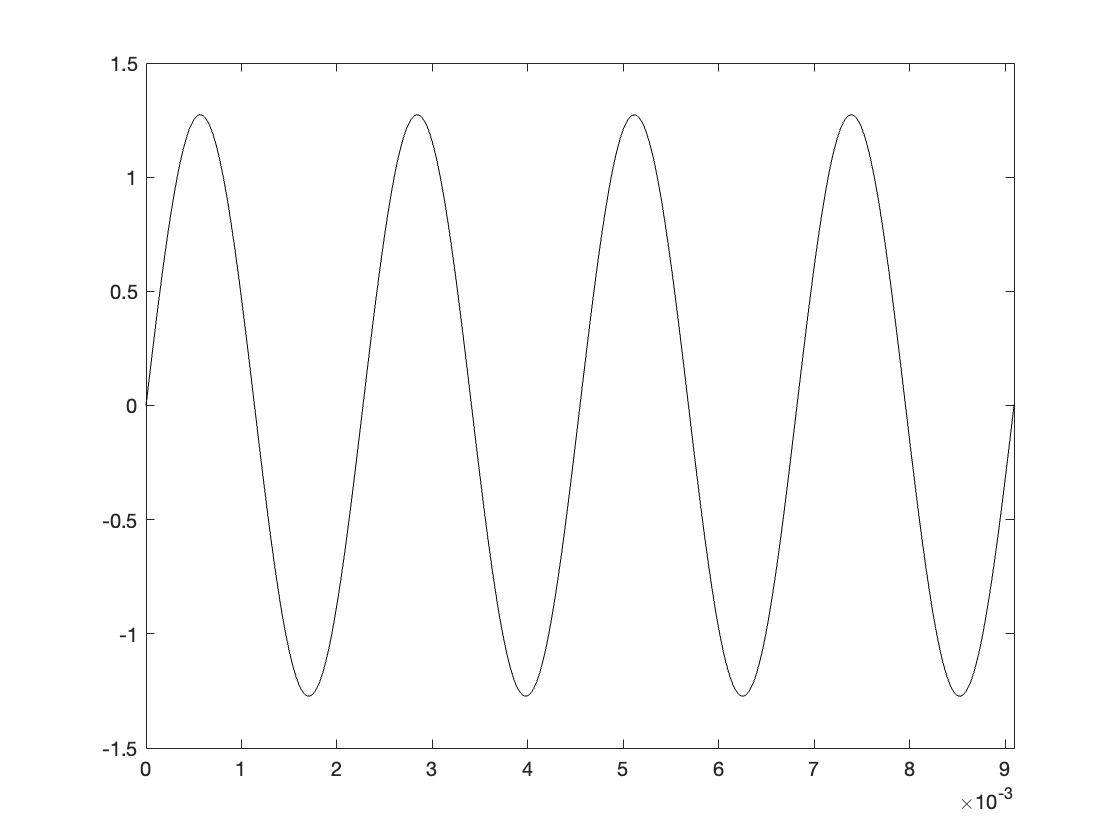
\includegraphics[scale=.18]{square_approx_1.png} & 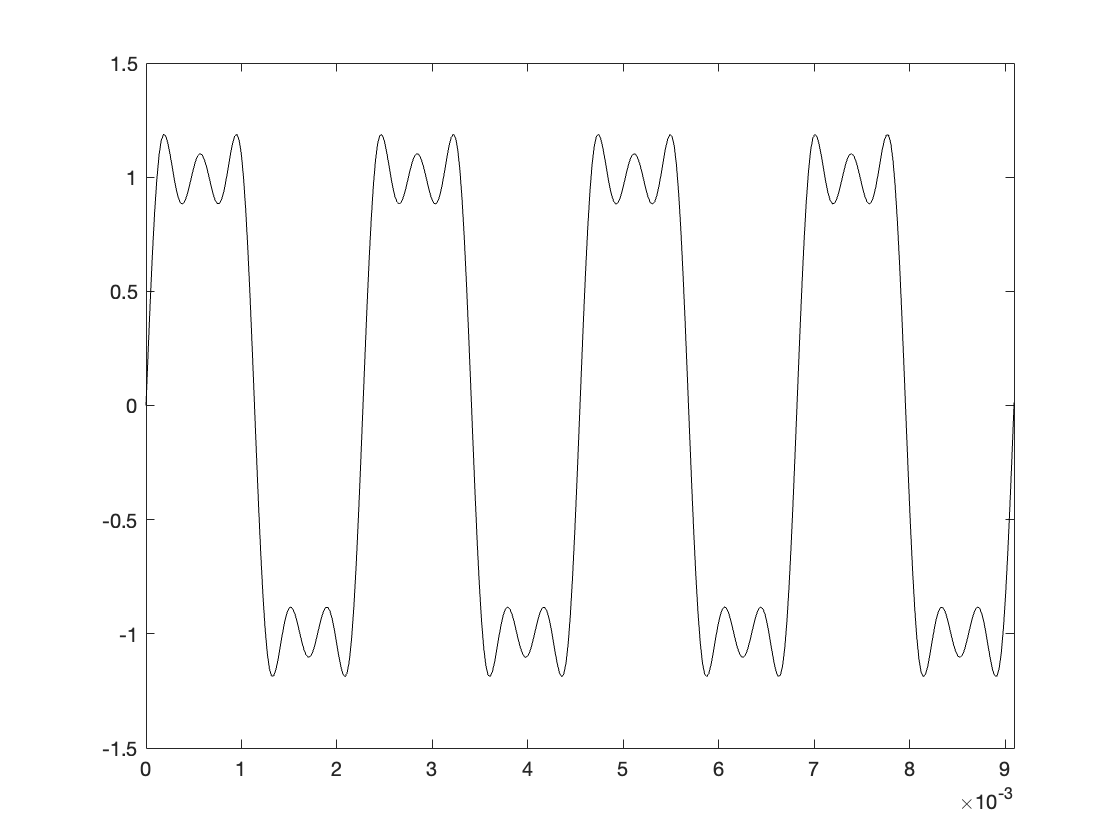
\includegraphics[scale=.18]{square_approx_5.png}\\
        \href{https://drive.google.com/file/d/1diLp3-edz0a5noPDrmdPAtLcfE1o02Mp/view?usp=sharing}{\color{blue} $[\blacktriangleright]~N = 1$} & \href{https://drive.google.com/file/d/1KRsDdJmrIZBzw05e9aXTSJ6JNP48DeH_/view?usp=sharing}{\color{blue}$[\blacktriangleright]~N = 5$}\\
        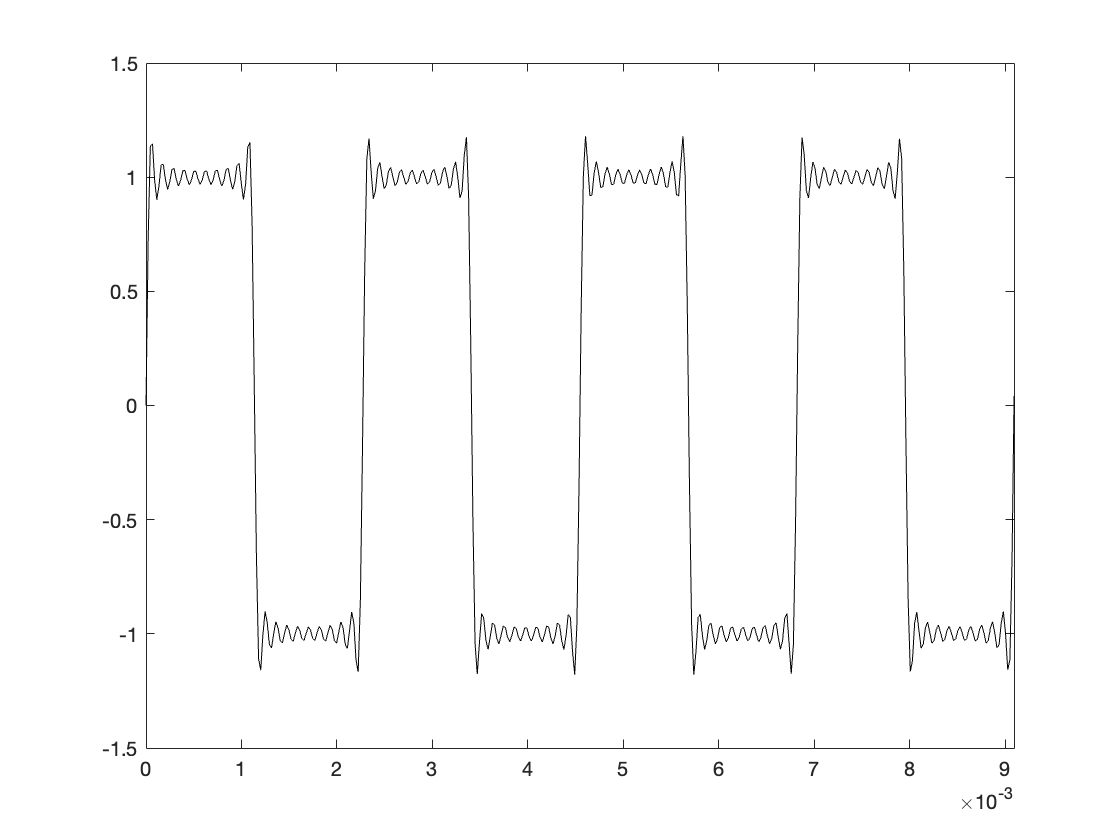
\includegraphics[scale=.18]{square_approx_20.png} & 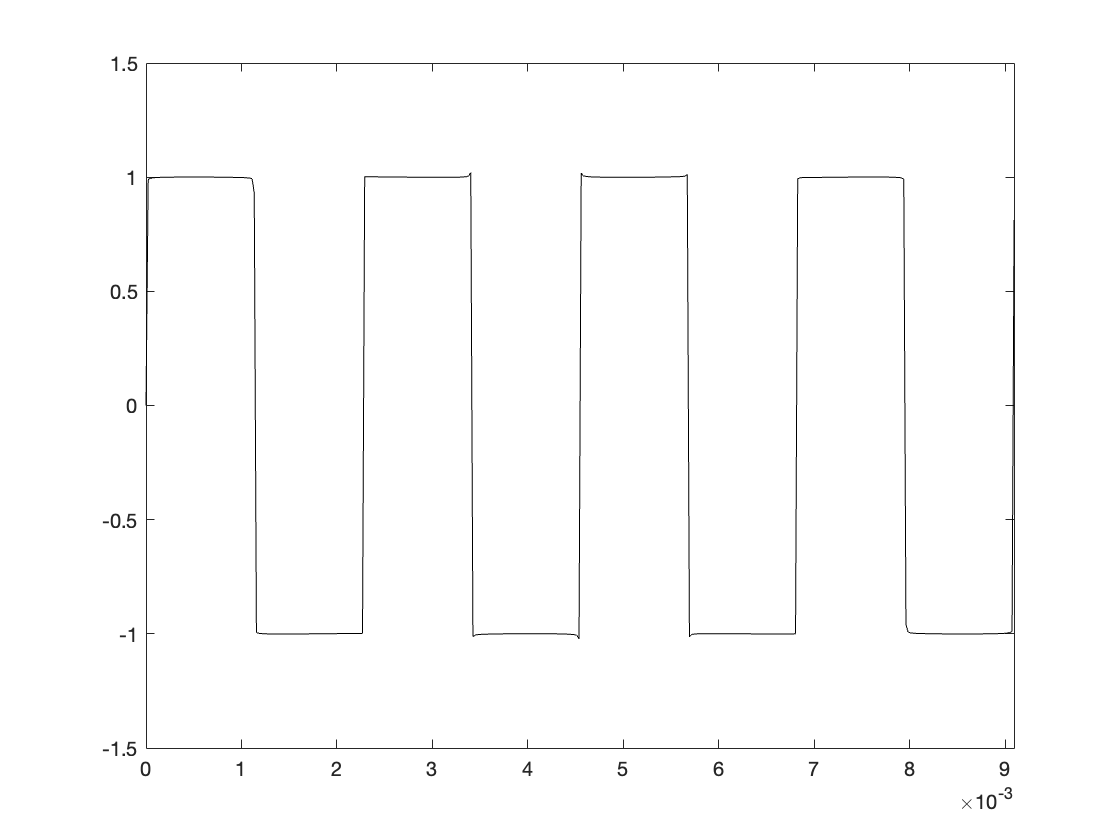
\includegraphics[scale=.18]{square_approx_1000.png}\\
        \href{https://drive.google.com/file/d/1Ke-h2uAj-fsGQuUQHSVxi4EvBqJfqqQg/view?usp=sharing}{\color{blue} $[\blacktriangleright]~N = 20$} & \href{https://drive.google.com/file/d/1kIVK22Os_Ny55Rpco6gKy--HNduItWO8/view?usp=sharing}{\color{blue}$[\blacktriangleright]~N = 1000$}\\
        
    \end{tabular}
    \caption{Fourier approximations of the square wave for A4}
    \label{fig:square_approx}
\end{figure}

\subsection{Linear Independence of the Real Fourier Terms}

\par \indentt The real Fourier terms span $\VNT$ because they are linearly independent. Proving the linear independence of Fourier terms for a general order $N$ is difficult. For now, we will prove linear independence for the case $N = 2$. Later, we will prove rigorously that the complex Fourier terms are linearly independent given any value of $N$.

\begin{theorem}
    Consider the second-order Fourier terms $\{1,\cos(\frac{2\pi t}{T}),\cos(\frac{4\pi t}{T}),\sin(\frac{2\pi t}{T}),\sin(\frac{4\pi t}{T})\}$. Let $a_0 + a_1\cos(\frac{2\pi t}{T}) + a_2\cos(\frac{4\pi t}{T}) + b_1\sin(\frac{2\pi t}{T}) + b_2\sin(\frac{4\pi t}{T}) = 0$. Then $a_0 = a_1 = a_2 = b_1 = b_2 = 0$. In other words, the second-order Fourier terms are linearly independent.
    
    \begin{proof}
        Let $t_1,t_2,t_3,t_4,t_5\in [0,T]$. Then we have the following system of equations:
        
        $$a_0 + a_1\cos(\frac{2\pi t_1}{T}) + a_2\cos(\frac{4\pi t_1}{T}) + b_1\sin(\frac{2\pi t_1}{T}) + b_2\sin(\frac{4\pi t_1}{T}) = 0$$
        $$a_0 + a_1\cos(\frac{2\pi t_2}{T}) + a_2\cos(\frac{4\pi t_2}{T}) + b_1\sin(\frac{2\pi t_2}{T}) + b_2\sin(\frac{4\pi t_2}{T}) = 0$$
        $$a_0 + a_1\cos(\frac{2\pi t_3}{T}) + a_2\cos(\frac{4\pi t_3}{T}) + b_1\sin(\frac{2\pi t_3}{T}) + b_2\sin(\frac{4\pi t_3}{T}) = 0$$
        $$a_0 + a_1\cos(\frac{2\pi t_4}{T}) + a_2\cos(\frac{4\pi t_4}{T}) + b_1\sin(\frac{2\pi t_4}{T}) + b_2\sin(\frac{4\pi t_4}{T}) = 0$$
        $$a_0 + a_1\cos(\frac{2\pi t_5}{T}) + a_2\cos(\frac{4\pi t_5}{T}) + b_1\sin(\frac{2\pi t_5}{T}) + b_2\sin(\frac{4\pi t_5}{T}) = 0.$$
        
        \par \bigskip Put in matrix form, this system is
        
        \[
        \begin{bmatrix}
            1 & \cos(\frac{2\pi t_1}{T}) & \cos(\frac{4\pi t_1}{T}) & \sin(\frac{2\pi t_1}{T}) & \sin(\frac{4\pi t_1}{T})\\
            1 & \cos(\frac{2\pi t_2}{T}) & \cos(\frac{4\pi t_2}{T}) & \sin(\frac{2\pi t_2}{T}) & \sin(\frac{4\pi t_2}{T})\\
            1 & \cos(\frac{2\pi t_3}{T}) & \cos(\frac{4\pi t_3}{T}) & \sin(\frac{2\pi t_3}{T}) & \sin(\frac{4\pi t_3}{T})\\
            1 & \cos(\frac{2\pi t_4}{T}) & \cos(\frac{4\pi t_4}{T}) & \sin(\frac{2\pi t_4}{T}) & \sin(\frac{4\pi t_4}{T})\\
            1 & \cos(\frac{2\pi t_5}{T}) & \cos(\frac{4\pi t_5}{T}) & \sin(\frac{2\pi t_5}{T}) & \sin(\frac{4\pi t_5}{T})\\
        \end{bmatrix} \begin{bmatrix}
            a_0\\
            a_1\\
            a_2\\
            b_1\\
            b_2\\
        \end{bmatrix} = 0.
        \]
        
        
        \par \bigskip If we can find 5 unique values of $t$ such that the row-reduced form of the square matrix above is the identity matrix, then all 5 coefficients must be 0.
        
        \par \bigskip Let $t_1 = 0$, $t_2 = \frac{T}{8}$, $t_3 = \frac{T}{4}$, $t_4 = \frac{T}{2}$, and $t_5 = \frac{3T}{4}$. Software tells us that
        
        \[
        \text{rref}\left(\begin{bmatrix}
            1 & \cos(0) & \cos(0) & \sin(0) & \sin(0)\\
            1 & \cos(\frac{\pi}{4}) & \cos(\frac{\pi}{2}) & \sin(\frac{\pi}{4}) & \sin(\frac{\pi}{2})\\
            1 & \cos(\frac{\pi}{2}) & \cos(\pi) & \sin(\frac{\pi}{2}) & \sin(\pi)\\
            1 & \cos(\pi) & \cos(2\pi) & \sin(\pi) & \sin(2\pi)\\
            1 & \cos(\frac{3\pi}{2}) & \cos(3\pi) & \sin(\frac{3\pi}{2}) & \sin(3\pi)\\
        \end{bmatrix}\right) = \text{rref}\left(\begin{bmatrix}
            1 & 1 & 1 & 0 & 0\\
            1 & \frac{1}{\sqrt{2}} & 0 & \frac{1}{\sqrt{2}} & 1\\
            1 & 0 & -1 & 1 & 0\\
            1 & -1 & 1 & 0 & 0\\
            1 & 0 & -1 & -1 & 0\\
        \end{bmatrix}\right) = I.
        \]
        
    \end{proof}
    \label{thm:real_F_lin_indep}
\end{theorem}

\par We can view the process of approximating $f(t)$ as a change of basis from the continuous-time domain, where coordinates are given by values of $t$, to the frequency domain $\VNT$, where coordinates are given by the Fourier coefficients found using the formulas in Definition \ref{real_F_coeffs} (i.e. the amplitudes of the pure tones that constitute $f(t)$).

\begin{definition}{The $N$'th-order real Fourier basis is the set of pure tones with frequency $\frac{n}{T}$ where $0\le n \le N$, notated as}
   \[\DNT = \left\{\begin{array}{ll}
   1,\cos(\frac{2\pi t}{T}), \cos(\frac{2\pi 2t}{T}), ..., \cos(\frac{2\pi Nt}{T}), \\
   \sin(\frac{2\pi t}{T}), \sin(\frac{2\pi 2t}{T}), ..., \sin(\frac{2\pi Nt}{T})
   \end{array}\right\}.\cite{Ryan}
   \]
\end{definition}